\section{Arquitectura de la propuesta de soluci�n}
Para garantizar niveles elevados de calidad de software durante el desarrollo es necesario definir desde el comienzo una arquitectura que describa sus principios fundamentales, garantizando robustez y escalabilidad.
La arquitectura de software define la estructura del sistema, la cual est� constituida por componentes, con funciones espec�ficas, que interact�an entre s� \citep{navarro2018arquitectura}.
\subsection{Patr�n Arquitect�nico}
Para el desarrollo de la propuesta de soluci�n se utiliza el patr�n arquitect�nico \ac{mvc} debido a que este separa la l�gica de negocio de la interfaz de usuario en tres capas diferentes, cada una con funcionalidades bien definidas, reduciendo esfuerzo en la implementaci�n de la aplicaci�n y garantizando una mejor organizaci�n del trabajo.
\subsubsection*{Partes del \ac{mvc}:}
\paragraph{ Modelo:} Contiene una representaci�n de los datos que maneja el sistema, su l�gica de negocio, y sus mecanismos de persistencia.
\paragraph{ Vista:} Tambi�n conocida como interfaz de usuario, compone la informaci�n que se env�a al cliente y los mecanismos de interacci�n con este.
\paragraph{ Controlador:} Act�a como intermediario entre el Modelo y la Vista, gestionando el flujo de informaci�n entre ellos y las transformaciones para adaptar los datos a las necesidades de cada uno.\\
\begin{figure}[htp]
	\centering
	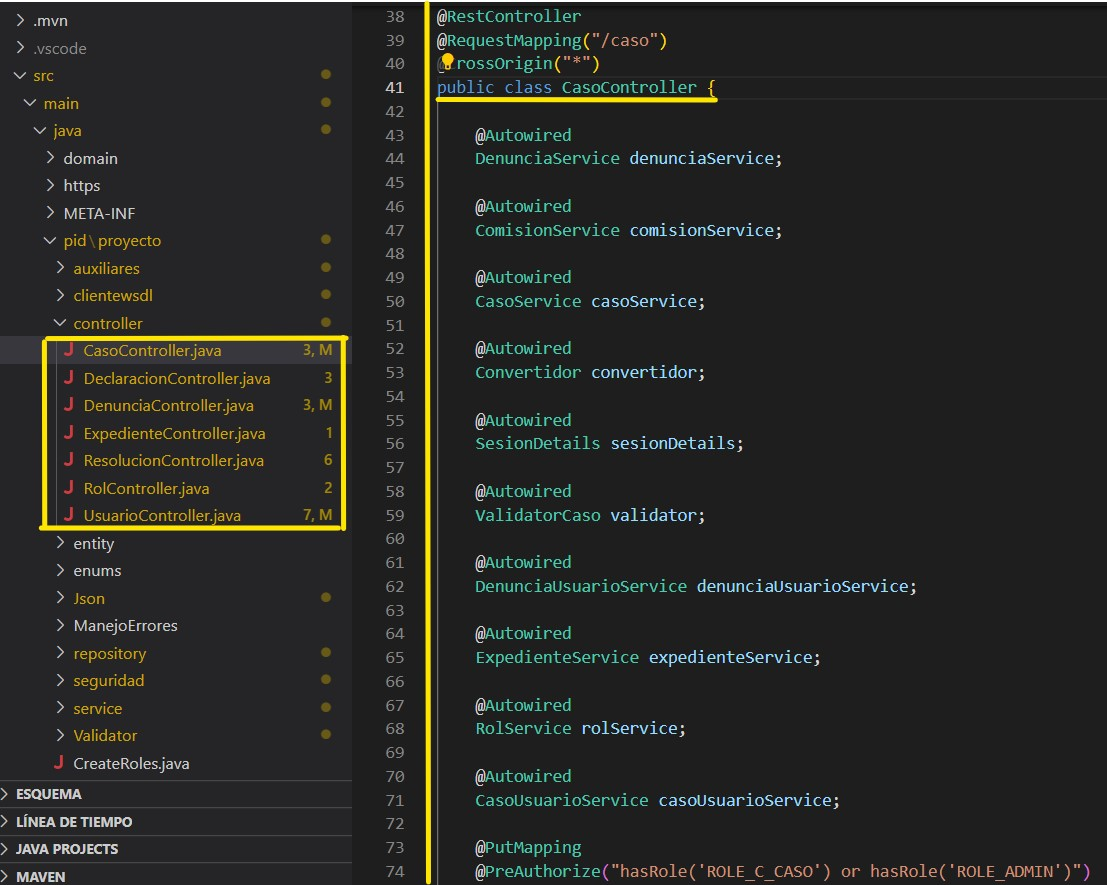
\includegraphics[width=0.5\textwidth]{images/patterns/controller.jpg}
	\caption{Ejemplo de la implmentaci�n de una clase controladora en el c�digo del sistema}
	\label{fig:arch-controller}
\end{figure}